% ChronoFuse — proje durum raporu (Türkçe). Derleme: tectonic proje_raporu.tex
\documentclass[11pt,a4paper]{article}
\usepackage{fontspec}           % XeTeX/tectonic: native Unicode (ş, ğ, ı, İ)
\usepackage[turkish]{babel}
\usepackage{microtype}
\usepackage[margin=2.3cm]{geometry}
\usepackage{booktabs,tabularx,array}
\usepackage{xcolor}
\usepackage{enumitem}
\usepackage{tikz}
\usetikzlibrary{babel,positioning,arrows.meta,fit,calc}
\usepackage[hidelinks]{hyperref}
\usepackage{fancyvrb}

\definecolor{ok}{HTML}{1A7F37}
\definecolor{wait}{HTML}{9A6700}
\definecolor{plan}{HTML}{6E7781}
\definecolor{accent}{HTML}{0B5CAD}
\newcommand{\OK}{\textcolor{ok}{\textbf{Çalıştırıldı}}}
\newcommand{\KOD}{\textcolor{wait}{\textbf{Kodlandı, çalıştırılmadı}}}
\newcommand{\PLAN}{\textcolor{plan}{\textbf{Planlandı}}}
\newcolumntype{L}{>{\raggedright\arraybackslash}X}
\setlist{itemsep=2pt,topsep=4pt}
\AtBeginDocument{\shorthandoff{=}}  % Turkish babel makes "=" active; breaks key=value options

\title{\textbf{ChronoFuse}\\[2pt]\large SemEval-2027 Task~1 (RETECO), Track~1 TEMPO için\\
zaman ve metadata farkındalıklı hibrit erişim\\[6pt]
\normalsize Proje Durum Raporu}
\author{Ahmet Önder Önlü \\ İstanbul Teknik Üniversitesi \\
\small Repo: \url{https://github.com/Ahmet-Onder-Onlu/nlp-term-project}}
\date{7 Kasım 2026}

\begin{document}
\maketitle

\begin{abstract}
\noindent Bu rapor dönem projesinin şu anki durumunu özetler: çözülen problemi, tasarlanan
sistemi (ChronoFuse), kullanılan araç ve kütüphaneleri, hangi modellerin kullanıldığını ve
şimdiye kadar alınan ölçülmüş çıktıları. Kısa durum: proje iskeleti ve tüm modüller yazıldı;
ancak şu ana kadar \emph{yalnızca BM25 kanalı} gerçek veride çalıştırıldı ve yalnızca
\emph{iota} domain'inde test edildi. Hiçbir embedding, reranker ya da LLM modeli henüz
indirilmedi veya çağrılmadı.
\end{abstract}

\tableofcontents
\newpage

%==========================================================================
\section{Problemin Tanımı}

\subsection{Görev}
RETECO (\emph{Reasoning-Oriented Retrieval}), SemEval-2027'nin 1 numaralı ortak görevidir
(Innsbruck Üniversitesi, UBC ve Johns Hopkins Üniversitesi tarafından düzenleniyor). İki ana
track ve beş alt görevden oluşur. Biz \textbf{Track~1: TEMPO (Temporal Grounded Retrieval)}
üzerinde çalışıyoruz:

\begin{itemize}
  \item \textbf{1a, Temporal Retrieval:} Karmaşık, zamana bağlı bir soru ve o domain'in doküman
        koleksiyonu verilir; sistem soru başına sıralı bir doküman listesi döndürür.
  \item \textbf{1b, Step-wise Temporal Retrieval:} Soru, akıl yürütme adımlarına bölünmüş olarak
        verilir; sistem her adım için ayrı bir sıralı liste döndürür.
\end{itemize}

Görevi zorlaştıran nokta şu: bir pasajın ilgili sayılması için hem \emph{konu} olarak hem de
\emph{zaman} olarak soruyla örtüşmesi gerekir. Doğru konuda ama yanlış dönemden bahseden bir
pasaj ilgili sayılmaz; görev sayfası da ilgisiz bir tarih içeren pasajın zamansal olarak
örtüşmüş sayılmadığını açıkça belirtiyor.

\paragraph{Örnek sorgu (iota domain'i).}
\begin{quote}\small
``Why are transactions so slow? Right now each transaction takes about 30 minutes or longer
\ldots{} two weeks ago the developers asked to stop the spamming \ldots''
\end{quote}
Burada zaman \emph{örtük} biçimde geçiyor (``right now'', ``two weeks ago''). Doğru cevap ise
belirli bir dönemdeki geliştirici duyurularına ve protokol belgelerine dayanıyor.

\subsection{Veri}
Veri, Hugging Face'teki \texttt{DataScience-UIBK/RETECO-SemEval2027} (v1.1) veri setidir.
Tüm metinler İngilizce StackExchange içeriğidir.

\begin{center}
\begin{tabular}{lr}
\toprule
Domain sayısı & 13 \\
Toplam doküman (v1.1, tekrarlar ayıklanmış) & 1.167.159 \\
Sorgu (train / dev) & 1.211 / 519 \\
Adım, 1b (train / dev) & 2.762 / 1.214 \\
Gizli test seti & yaklaşık 350 sorgu \\
\bottomrule
\end{tabular}
\end{center}

\noindent Domain'ler: bitcoin, cardano, iota, monero (blockchain); economics, law, politics,
history (sosyal bilimler); quant, travel, workplace, genealogy (uygulamalı); hsm (bilim ve
matematik tarihi). Her domain'in kendi doküman koleksiyonu vardır; train ve dev 70/30 oranında
bölünmüştür.

\paragraph{Guidance dosyaları.}
Train ve dev sorguları için \texttt{guidance\_*.jsonl} dosyaları her sorgunun zamansal
etiketlerini içerir: zamansal niyet (ör.\ \texttt{ongoing\_status}), beklenen zaman
granülaritesi, zaman çapaları, olaylar ve adım adım bir arama planı. \textbf{Test setinde bu
dosyalar yok.} Tasarımımızın merkezindeki fikirlerden biri, bu etiketleri LLM'e örnek
(few-shot) olarak vererek aynı şemayı test sorguları için tahmin ettirmek
(Bölüm~\ref{sec:sistem}).

\subsection{Değerlendirme}
\begin{itemize}
  \item \textbf{Resmi metrik:} \texttt{pytrec\_eval} ile ikili nDCG@10. Önce her domain'in
        ortalaması alınır, sonra 13 domain'in ortalaması (macro-average).
  \item Run dosyasında eksik kalan sorgu 0 puan alır. Gönderim formatı altı sütunlu TREC
        formatıdır.
  \item \textbf{Teşhis metrikleri} (sıralamaya girmez): Temporal Precision@10, Temporal
        Relevance@10, Temporal Coverage@10, NDCG|FC@10.
  \item \textbf{Resmi BM25 baseline'ı}, macro nDCG@10:
        1a train / dev = 0,1075 / 0,1147; 1b train / dev = 0,1024 / 0,1177.
\end{itemize}
Bu düşük skorlar, salt anahtar kelime eşleşmesinin bu görevde yetersiz kaldığını ve iyileştirme
için geniş bir alan olduğunu gösteriyor.

\subsection{Takvim}
Değerlendirme penceresi 10 Ocak 2027'de açılıp en geç 31 Ocak 2027'de kapanıyor. Makale
gönderimi Şubat 2027'de (tahmini) ve ACL formatında olacak.

%==========================================================================
\section{Çözüm: ChronoFuse}
\label{sec:sistem}

\subsection{Genel mimari}

\begin{center}
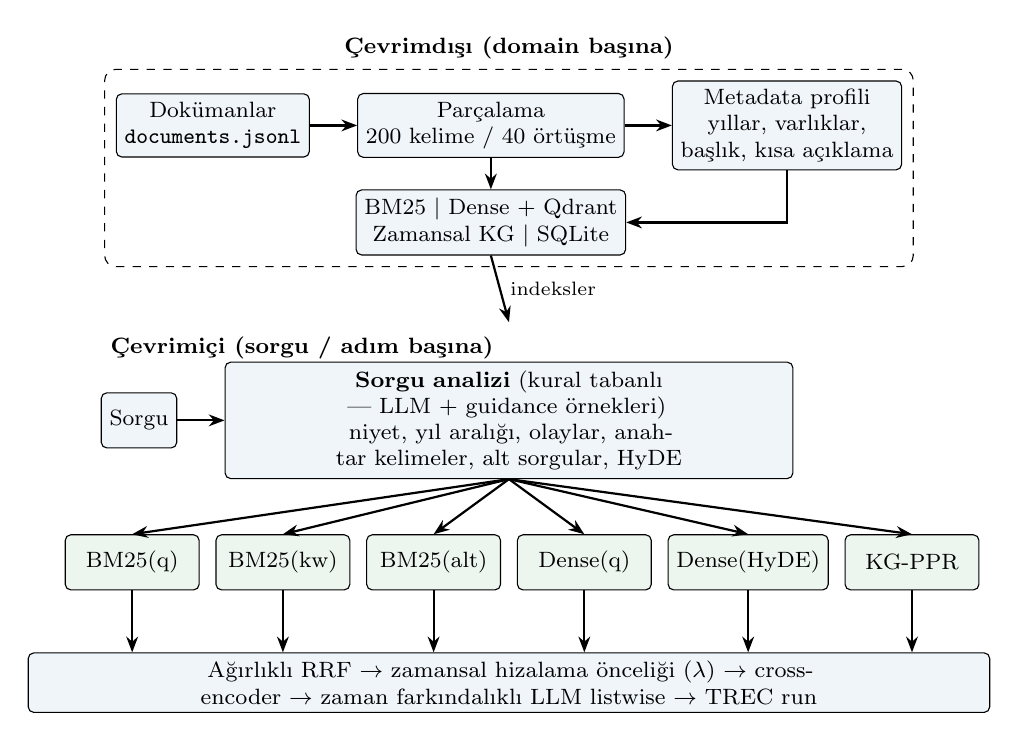
\begin{tikzpicture}[
  font=\footnotesize,
  box/.style={draw, rounded corners=2pt, align=center, minimum height=7mm, inner sep=3pt,
              fill=accent!6},
  ch/.style={box, fill=ok!8, minimum width=17mm},
  arr/.style={-{Stealth[length=2mm]}, thick}]
  % offline
  \node[box] (docs) {Dokümanlar\\\texttt{documents.jsonl}};
  \node[box, right=6mm of docs] (chunk) {Parçalama\\200 kelime / 40 örtüşme};
  \node[box, right=6mm of chunk] (meta) {Metadata profili\\yıllar, varlıklar,\\başlık, kısa açıklama};
  \node[box, below=4mm of chunk] (idx) {BM25 \textbar{} Dense + Qdrant\\Zamansal KG \textbar{} SQLite};
  \draw[arr] (docs) -- (chunk); \draw[arr] (chunk) -- (meta); \draw[arr] (chunk) -- (idx);
  \draw[arr] (meta) |- (idx);
  \node[draw, dashed, rounded corners, inner sep=4pt, fit=(docs)(chunk)(meta)(idx),
        label={[font=\footnotesize\bfseries]above:Çevrimdışı (domain başına)}] (off) {};
  % online
  \node[box, text width=70mm, anchor=north] (qa) at ($(off.south)+(0,-12mm)$)
       {\textbf{Sorgu analizi} (kural tabanlı | LLM + guidance örnekleri)\\
        niyet, yıl aralığı, olaylar, anahtar kelimeler, alt sorgular, HyDE};
  \node[box, left=6mm of qa] (q) {Sorgu};
  \draw[arr] (q) -- (qa);
  \draw[arr] (idx.south) -- node[right, font=\scriptsize]{indeksler} ($(off.south)+(0,-7mm)$);
  \node[ch, anchor=north east] (c3) at ($(qa.south)+(-1mm,-7mm)$) {BM25(alt)};
  \node[ch, left=2mm of c3] (c2) {BM25(kw)};
  \node[ch, left=2mm of c2] (c1) {BM25(q)};
  \node[ch, anchor=north west] (c4) at ($(qa.south)+(1mm,-7mm)$) {Dense(q)};
  \node[ch, right=2mm of c4] (c5) {Dense(HyDE)};
  \node[ch, right=2mm of c5] (c6) {KG-PPR};
  \foreach \c in {c1,c2,c3,c4,c5,c6} \draw[arr] (qa.south) -- (\c.north);
  \node[box, text width=120mm, anchor=north] (fuse) at ($(qa.south)+(0,-22mm)$)
       {Ağırlıklı RRF $\rightarrow$ zamansal hizalama önceliği ($\lambda$)
        $\rightarrow$ cross-encoder $\rightarrow$ zaman farkındalıklı LLM listwise
        $\rightarrow$ TREC run};
  \foreach \c in {c1,c2,c3,c4,c5,c6} \draw[arr] (\c.south) -- (fuse.north -| \c.south);
  \node[font=\footnotesize\bfseries, anchor=south west] at ($(q.north west)+(0,3mm)$)
       {Çevrimiçi (sorgu / adım başına)};
\end{tikzpicture}
\end{center}

\subsection{Bileşenler ve durumları}
Aşağıdaki tabloda her bileşenin kodda bulunduğu yer ve şu anki durumu var. ``Çalıştırıldı'',
gerçek RETECO verisinde ölçüldüğü anlamına geliyor.

\medskip
\noindent\begin{tabularx}{\textwidth}{>{\raggedright\arraybackslash}p{3.6cm} L >{\raggedright\arraybackslash}p{2.9cm}}
\toprule
\textbf{Bileşen} & \textbf{Ne yapıyor} & \textbf{Durum} \\
\midrule
Veri yükleyici \newline\scriptsize\texttt{data/reteco.py} &
  Sorgu, adım, guidance, qrels ve doküman koleksiyonunu okur; sorgulardaki HTML'i temizler. & \OK \\
Parçalama + MaxP \newline\scriptsize\texttt{metadata/chunking.py} &
  Dokümanları örtüşmeli pasajlara böler (en fazla 64 pasaj); doküman skoru, pasaj skorlarının
  en yükseğidir. & \OK \\
Zamansal ifade çıkarımı \newline\scriptsize\texttt{metadata/temporal.py} &
  Yıl, yıl aralığı, ay-yıl, ISO tarih, onyıl, yüzyıl ve göreli ifadeleri (``two weeks ago'')
  bulur ve yıllara normalize eder. & \OK{} \newline\scriptsize(birim testli) \\
Doküman profili \newline\scriptsize\texttt{metadata/profile.py} &
  Her doküman için başlık, kısa açıklama, yıllar, granülarite ve varlıkları JSONL dosyasına
  yazar. & \OK{} \newline\scriptsize(iota için üretildi) \\
BM25 \newline\scriptsize\texttt{indexing/bm25\_index.py} &
  \texttt{bm25s} ile Lucene tipi BM25 ($k_1{=}0{,}9$, $b{=}0{,}4$), İngilizce stemmer. & \OK \\
SQLite doküman deposu \newline\scriptsize\texttt{store.py} &
  Reranker'ların doküman metnine hızlı erişmesi için. & \OK \\
Değerlendirme \newline\scriptsize\texttt{eval/metrics.py} &
  Resmi kurala uygun nDCG@10 (eksik sorgu 0 puan), recall@100, TREC yazma ve okuma. & \OK{}
  \newline\scriptsize(resmi scorer ile birebir) \\
Dense erişim \newline\scriptsize\texttt{indexing/dense\_index.py} &
  sentence-transformers ile embedding, FAISS ile iç çarpım araması. & \KOD \\
Vektör veritabanı \newline\scriptsize\texttt{indexing/vector\_store.py} &
  Qdrant; payload'da yıllar tutulur, sorgunun yıl aralığına göre filtreleme yapılabilir. & \KOD \\
Zamansal bilgi grafiği \newline\scriptsize\texttt{kg/temporal\_kg.py} &
  Doküman, varlık ve yıl düğümleri; kişiselleştirilmiş PageRank ile erişim. İsteğe bağlı
  Neo4j'ye aktarım. & \KOD \\
Sorgu analizcisi \newline\scriptsize\texttt{query/analyzer.py} &
  Kural tabanlı sürüm ve guidance örnekleriyle çalışan LLM sürümü (JSON çıktı). & Kural: \OK
  \newline LLM: \KOD \\
Füzyon + zamansal öncelik \newline\scriptsize\texttt{retrieval/} &
  Ağırlıklı RRF ve CombSUM; $s' = (1-\lambda)\hat s + \lambda\,T(q,d)$. & \KOD{}
  \newline\scriptsize(RRF birim testli) \\
Cross-encoder \newline\scriptsize\texttt{rerank/cross\_encoder.py} &
  Adayları ``[yıllar] başlık --- pasaj'' biçiminde metadata ile zenginleştirip yeniden
  sıralar. & \KOD \\
LLM listwise reranker \newline\scriptsize\texttt{rerank/llm\_listwise.py} &
  RankGPT tarzı kayan pencere; prompt'ta sorgunun zamansal ihtiyacı yer alır. & \KOD \\
RAPTOR tarzı küme özetleri & Domain içi hiyerarşik özetlerden ek bir erişim kanalı. & \PLAN \\
\bottomrule
\end{tabularx}

\subsection{Özgün katkı fikirleri}
\begin{enumerate}
  \item \textbf{Guidance distillation:} Benchmark'ın yalnızca train ve dev için verdiği zamansal
        etiket şemasını LLM'e örnek olarak verip test sorguları için aynı şemayı ürettirmek.
        Analizcinin doğruluğu dev setinde gerçek guidance ile karşılaştırılarak ölçülebilir.
  \item \textbf{Metadata'nın her aşamada kullanılması:} Aynı zamansal profil KG'de, vektör
        veritabanı filtresinde, zamansal öncelik skorunda ve reranker prompt'larında kullanılır.
  \item \textbf{Çok kanallı hibrit erişim ve ablation:} Altı kanal tek tek açılıp kapatılarak
        her birinin katkısı ölçülecek.
\end{enumerate}

%==========================================================================
\section{Kullanılan Araç ve Kütüphaneler}

\noindent\begin{tabularx}{\textwidth}{>{\raggedright\arraybackslash}p{3.8cm} L >{\raggedright\arraybackslash}p{2.9cm}}
\toprule
\textbf{Araç} & \textbf{Rolü} & \textbf{Durum} \\
\midrule
Python 3.11, conda/mamba & Çalışma ortamı (\texttt{reteco}) & \OK \\
PyTorch 2.15 (CPU sürümü) & Sinir ağı modelleri için altyapı (makinede GPU yok) & Kuruldu \\
\texttt{bm25s} + PyStemmer & Seyrek (sparse) erişim, BM25 & \OK \\
\texttt{pytrec\_eval} & Resmi nDCG@10 hesabı & \OK \\
SQLite, \texttt{orjson} & Doküman deposu, hızlı JSON okuma & \OK \\
Hugging Face Hub & Veri indirme & \OK \\
RETECO starter kit & Resmi \texttt{scorer.py} ve \texttt{format\_checker.py} ile çapraz kontrol & \OK \\
sentence-transformers, FAISS & Dense erişim ve cross-encoder & \KOD \\
Qdrant (gömülü mod) & Metadata filtreli vektör veritabanı & \KOD \\
NetworkX / Neo4j & Bilgi grafiği (bellek içi / harici) & \KOD \\
OpenAI uyumlu istemci & LLM çağrıları (OpenAI, vLLM, Ollama, OpenRouter); disk önbellekli & \KOD \\
pytest, ruff & 8 birim testi, lint ve biçimlendirme & \OK \\
Git, GitHub CLI & Sürüm kontrolü, public repo & \OK \\
LaTeX (ACL stili), tectonic & Makale ve bu rapor & \OK \\
\bottomrule
\end{tabularx}

%==========================================================================
\section{Modeller: Neler İndirildi, Neler Kullanıldı?}
\label{sec:modeller}

\textbf{Kısa cevap: henüz hiçbir model indirilmedi ve hiçbir LLM çağrılmadı.} Şimdiye kadarki
tüm sonuçlar BM25'e dayanıyor; BM25 bir istatistiksel sıralama fonksiyonu, öğrenilmiş bir model
değil. Hugging Face model önbelleği kontrol edildi ve boş. Kodda tanımlı olan
\emph{varsayılan} seçimler şunlar:

\medskip
\noindent\begin{tabularx}{\textwidth}{>{\raggedright\arraybackslash}p{2.9cm} >{\raggedright\arraybackslash}p{5.0cm} L}
\toprule
\textbf{Rol} & \textbf{Varsayılan model} & \textbf{Durum ve not} \\
\midrule
Embedding (dense) & \texttt{BAAI/bge-small-en-v1.5} & İndirilmedi. CPU'da hızlı olduğu için
  seçildi; son sistemde GPU'da daha güçlü bir model (ör.\ \texttt{bge-m3}) düşünülüyor. \\
Cross-encoder reranker & \texttt{BAAI/bge-reranker-v2-m3} & İndirilmedi. \\
LLM (sorgu analizi + rerank) & \texttt{.env} içindeki \texttt{LLM\_MODEL} (örnek dosyadaki
  varsayılan: \texttt{gpt-4o-mini}) & \textbf{Henüz seçilmedi.} API anahtarı yok, hiç çağrı
  yapılmadı. Hangi model ve servisin (API mi, yerel Ollama mı) kullanılacağına birlikte karar
  verilecek. \\
\bottomrule
\end{tabularx}

\paragraph{Donanım kısıtı.} Makinede GPU yok ve 7,6~GB RAM var. 1,17 milyon dokümanı CPU'da
embedding'e çevirmek saatler sürer. Bu yüzden dense indeksleme için Colab/Kaggle GPU'su ya da
küçük bir model gerekecek.

%==========================================================================
\section{Çıktılar (Ölçülmüş Sonuçlar)}

\subsection{Duman testi: iota domain'i, E0 (pasaj BM25 + MaxP)}
iota domain'inde 9.680 doküman ve 21.403 pasaj var. İndeks 12 saniyede kuruldu ve en fazla
yaklaşık 340~MB bellek kullandı.

\begin{center}
\begin{tabular}{lcccc}
\toprule
& \textbf{Sorgu / adım} & \textbf{Bizim E0} & \textbf{Resmi BM25 (iota)} & \textbf{Recall@100} \\
\midrule
1a train & 7  & 0,3159 & 0,1563 & 0,500 \\
1a dev   & 3  & 0,4895 & 0,3309 & 1,000 \\
1b train & 16 & 0,1980 & 0,1403 & 0,719 \\
1b dev   & 8  & 0,4539 & 0,4195 & 0,750 \\
\bottomrule
\end{tabular}
\end{center}

\paragraph{Resmi scorer ile çapraz kontrol (1a).} Organizatörlerin \texttt{scorer.py} betiği
bizim değerlendirmemizle aynı nDCG@10 değerlerini verdi; \texttt{format\_checker.py} de run
dosyaları için \texttt{VALID} sonucunu döndü. Resmi scorer'ın teşhis metrikleri:

\begin{center}
\begin{tabular}{lccccc}
\toprule
& nDCG@10 & TP@10 & TR@10 & TC@10 & NDCG|FC@10 \\
\midrule
1a train & 0,3159 & 0,1588 & 0,1143 & 0,4524 & 0,5585 \\
1a dev   & 0,4895 & 0,2518 & 0,1667 & 0,5000 & 0,7031 \\
\bottomrule
\end{tabular}
\end{center}

\paragraph{Yorum ve uyarı.} Bizim E0, iota'da resmi baseline'dan yüksek çıktı. Ancak bu henüz
bir başarı iddiası \emph{değil}: (i)~iota'da yalnızca 7 train ve 3 dev sorgusu var, bu yüzden
sonuçlar çok oynak; (ii)~E0, resmi baseline'ın birebir kopyası değil (parçalama, stemmer ve
tokenizer farklı). Asıl karşılaştırma 13 domain'in macro ortalamasıyla yapılacak.

\subsection{Üretilen dosyalar}
\begin{itemize}
  \item \texttt{results/runs/e0\_bm25/\{1a,1b\}\_\{train,dev\}/iota.trec}: TREC run dosyaları
  \item \texttt{results/metrics/e0\_bm25\_\_*.json}: domain bazında metrikler
  \item \texttt{data/indexes/iota/}: BM25 indeksi, metadata profilleri, SQLite deposu
  \item \texttt{paper/main.pdf}: ACL formatında makale iskeleti (4 sayfa, sonuçlar boş)
\end{itemize}

%==========================================================================
\section{LaTeX Çıktısını Görme}
İki yol var:
\begin{enumerate}
  \item \textbf{Overleaf:} \texttt{paper/} klasörünü zip'leyip Overleaf'te
        \emph{New Project $\rightarrow$ Upload Project} ile yükleyin; derleyici pdfLaTeX olarak
        kalabilir. Klasördeki \texttt{acl.sty}, \texttt{acl\_natbib.bst}, \texttt{sections/}
        ve iki \texttt{.bib} dosyası yeterli.
  \item \textbf{Yerelde:} \texttt{reteco} ortamına \texttt{tectonic} kuruldu:
\begin{Verbatim}[fontsize=\small,frame=single]
conda activate reteco
cd paper && tectonic main.tex                  # -> paper/main.pdf
cd reports && tectonic proje_raporu.tex        # -> bu rapor
\end{Verbatim}
\end{enumerate}

%==========================================================================
\section{Sonraki Adımlar}
\begin{enumerate}
  \item 13 domain'in tamamını indirmek (yaklaşık 2~GB) ve E0'ı resmi macro baseline ile
        karşılaştırmak. Bitcoin domain'i büyük olduğundan, 7,6~GB RAM'de indekslemeyi parça
        parça (batch) yapmak gerekebilir.
  \item Metadata analizi: dokümanların yıl içerme oranı ve guidance'taki zamansal niyet dağılımı.
  \item E1 (zamansal öncelik, $\lambda$ train'de ayarlanacak) $\rightarrow$ E2 (dense + KG)
        $\rightarrow$ E3 (LLM analizi + reranking).
  \item LLM ve embedding modeline karar vermek (API maliyeti ve GPU erişimine göre).
  \item Ablation, domain ve niyet bazlı analizler; makalenin yazılması.
\end{enumerate}

\end{document}
